% SCIENCE Visual Guide 2.0.1 + AI_SKILLS_R5; Akulin--Karlov batch v2.
% Graph traces are visibly heavier than axes. All labels use anchored positions.
\documentclass[border=5pt]{standalone}
\usepackage{fontspec,unicode-math}
\setmainfont{Noto Sans}
\setsansfont{Noto Sans}
\setmathfont{STIXTwoMath-Regular.otf}
\usepackage{tikz}
\usetikzlibrary{arrows.meta,calc,patterns,decorations.pathreplacing,intersections}
\definecolor{ScienceInk}{HTML}{000000}
\definecolor{ScienceCurve}{HTML}{000000}
\definecolor{ScienceAux}{HTML}{000000}
\definecolor{ScienceMuted}{HTML}{000000}
\tikzset{
  axis/.style={draw=ScienceInk,line width=0.75pt,-{Latex[length=2.2mm,width=1.35mm]}},
  axisplain/.style={draw=ScienceInk,line width=0.70pt},
  curve/.style={draw=ScienceCurve,line width=2.15pt,line cap=round,line join=round},
  curveb/.style={draw=ScienceAux,line width=1.95pt,dash pattern=on 6pt off 2.4pt,line cap=round,line join=round},
  curvedash/.style={draw=ScienceAux,line width=1.9pt,dash pattern=on 4pt off 3pt},
  optbeam/.style={draw=ScienceCurve,line width=1.75pt,-{Latex[length=2.2mm,width=1.3mm]}},
  optback/.style={draw=ScienceAux,line width=1.65pt,-{Latex[length=2mm,width=1.2mm]}},
  opt/.style={draw=ScienceInk,line width=1.0pt},
  opticplate/.style={draw=ScienceInk,line width=1.02pt,pattern=north east lines,pattern color=ScienceMuted},
  tick/.style={draw=ScienceInk,line width=0.7pt},
  textlabel/.style={text=ScienceInk,font=\fontsize{15}{18}\selectfont},
  smalllabel/.style={text=ScienceInk,font=\fontsize{13.5}{16.2}\selectfont},
}
\begin{document}
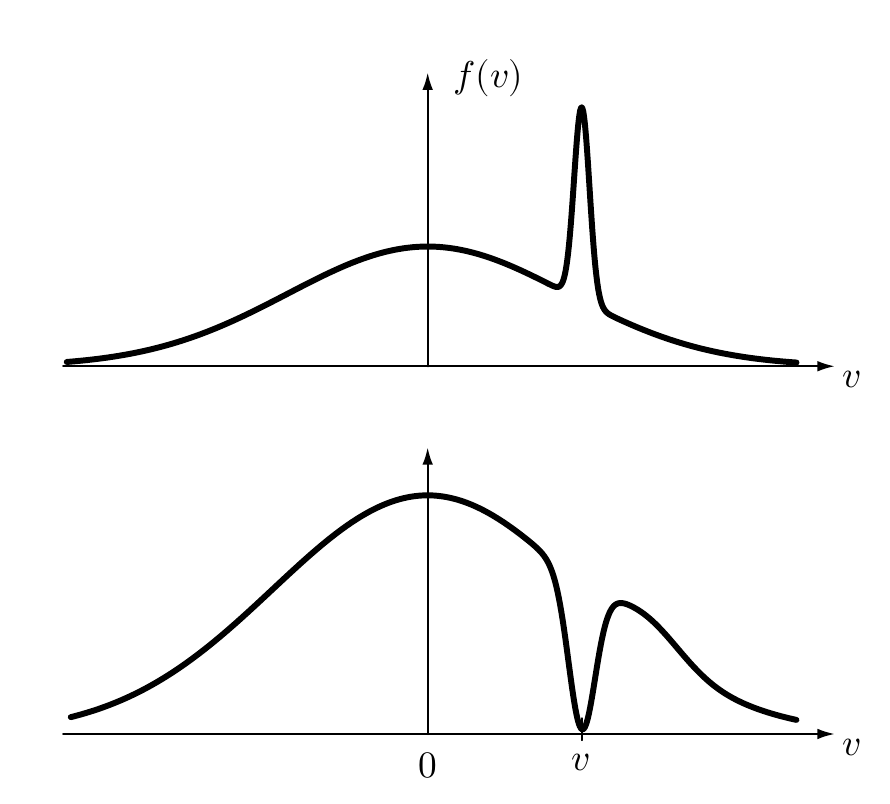
\begin{tikzpicture}[x=1cm,y=1cm,>=Latex,line cap=round,line join=round,font=\fontsize{15}{18}\selectfont]


\path[use as bounding box] (0,0) rectangle (10.6,9.5);
\begin{scope}[shift={(0,4.68)}]
\draw[axis] (.45,.52)--(10.25,.52);
\draw[axis] (5.08,.52)--(5.08,4.25);
\node[smalllabel,anchor=west] at (5.29,4.18) {$f(v)$};
\node[smalllabel,anchor=west] at (10.22,.35) {$v$};
\draw[curve,samples=480,domain=-4.45:4.55,smooth] plot ({5.08+1.03*\x},{.52+1.52*exp(-(.41*\x)^2)+2.46*exp(-((\x-1.90)/.135)^2)});
\end{scope}
\begin{scope}[shift={(0,.05)}]
\draw[axis] (.45,.48)--(10.25,.48);
\draw[axis] (5.08,.48)--(5.08,4.12);
\node[smalllabel,anchor=west] at (10.22,.31) {$v$};
\draw[curve,samples=550,domain=-4.4:4.55,smooth] plot ({5.08+1.03*\x},{.48+3.03*exp(-(.37*\x)^2)-1.86*exp(-((\x-1.90)/.23)^2)+.38*exp(-((\x-2.70)/.62)^2)});
\draw[tick] ({5.08+1.03*1.90},.40)--({5.08+1.03*1.90},.68);
\node[smalllabel,anchor=north] at ({5.08+1.03*1.90},.35) {$v_{\mathrm{рез}}$};
\node[smalllabel,anchor=north] at (5.08,.37) {$0$};
\end{scope}

\end{tikzpicture}
\end{document}
